% ======================================================================
% Deliverable 3: Final Report  --  Machine Learning (101700), IBA
% Compile with XeLaTeX (or upload this folder to Overleaf, compiler XeLaTeX).
% ======================================================================
\PassOptionsToPackage{unicode}{hyperref}
\PassOptionsToPackage{hyphens}{url}
\documentclass[11pt]{article}
\usepackage{amsmath,amssymb}
\usepackage{iftex}
\ifPDFTeX
  \usepackage[T1]{fontenc}
  \usepackage[utf8]{inputenc}
  \usepackage{textcomp}
  \usepackage{lmodern}
\else
  \usepackage{unicode-math}
  \defaultfontfeatures{Scale=MatchLowercase}
  \defaultfontfeatures[\rmfamily]{Ligatures=TeX,Scale=1}
  \setmainfont[]{Latin Modern Roman}
\fi
\IfFileExists{upquote.sty}{\usepackage{upquote}}{}
\usepackage[]{microtype}
\usepackage{parskip}
\usepackage{xcolor}
\usepackage[margin=0.9in]{geometry}
\usepackage{booktabs,array,longtable,tabularx}
\newcolumntype{L}[1]{>{\raggedright\arraybackslash}p{#1}}
\newcolumntype{Y}{>{\raggedright\arraybackslash}X}
\usepackage{graphicx}
\usepackage{float}
\usepackage[font=small,labelfont=bf,skip=4pt]{caption}
\usepackage{enumitem}
\setlist{itemsep=2pt,topsep=3pt}
\usepackage{algorithm}
\usepackage{algpseudocode}
\usepackage{tikz}
\usetikzlibrary{arrows.meta,positioning,fit,calc}
\usepackage[most]{tcolorbox}
\usepackage{listings}
\lstset{basicstyle=\ttfamily\small,columns=fullflexible,breaklines=true,frame=single,
        framerule=0.3pt,rulecolor=\color{black!30},backgroundcolor=\color{black!3},
        xleftmargin=4pt,xrightmargin=4pt,aboveskip=6pt,belowskip=6pt}
\usepackage{xurl}
\usepackage{bookmark}
\urlstyle{same}
\hypersetup{hidelinks,pdftitle={Deliverable 3: Final Report -- OCTree on the Electricity Dataset}}
\setcounter{secnumdepth}{3}
\setlength{\emergencystretch}{3em}

\newcommand{\code}[1]{\texttt{#1}}
% ---- Repository link shown on the title page: replace the text between the braces ----
\newcommand{\githublink}{\url{https://github.com/Shehryar-Arshad/OCTREE-Electricity-Reproduction}}

\begin{document}

% ---------------------------------------------------------------------- title page
\begin{titlepage}
\noindent\hfill\includegraphics[width=1.35in]{media/image1.jpg}\par
\centering\vspace*{1.2cm}
{\huge\bfseries Final Report\par}
\vspace{0.8cm}
{\Large Optimized Feature Generation for Tabular Data via\\[2pt]
LLMs with Decision Tree Reasoning:\\[4pt]
\textit{A Reproduction on the Electricity Dataset}\par}
\vspace{1.0cm}
{\large Machine Learning (101700)\par}
\vspace{1.4cm}
{\large Submitted to: Dr. Rizwan Ahmed Khan\par}
\vspace{1.2cm}
Submitted by:\par\medskip
{\large Muhammad Salman Malik -- 36403\par\medskip
Muhammad Shehryar Arshad -- 36220\par\medskip
Manahil Imran -- 36400\par}
\vfill
{\large GitHub link: \githublink\par}
\vspace{0.6cm}
\end{titlepage}

\tableofcontents
\clearpage

% ======================================================================
\section{Introduction and Problem Statement}\label{sec:intro}

Tabular data, records organized into rows of observations and columns of various numeric and
categorical features, is the most common data format used in the healthcare, finance, education and
business sectors. Despite the successes of deep learning on text and images, gradient-boosted decision
trees remain the leading approach for the bulk of tabular prediction tasks (Grinsztajn et al., 2022).
Practitioners continue to rely on feature engineering to extract additional benefits. New features
can be handcrafted, but this is costly and requires domain knowledge, and current automated
approaches can only explore a limited, pre-defined space of transformations and rely on a single
validation criterion (Nam et al., 2024).

\subsection{Problem Statement}
Given a tabular dataset with columns $x_1,\dots,x_M$ and a target $y$, the task is to find a rule
that computes a new column $x_{M+1}=r(x_1,\dots,x_M)$ such that a prediction model trained on the
augmented data generalizes better than one trained on the original columns. The difficulty is that
the space of possible rules is effectively unlimited, every candidate must be checked by training a
model, and, when the columns are anonymized, no domain knowledge is available to guide the search.

Nam et al. (2024) address this problem with OCTree (Optimizing Column feature generator with
decision Tree reasoning), which uses a large language model (LLM) as an optimizer. The LLM proposes
a rule that generates a new column, a prediction model is trained on the augmented data, and both
the validation score and a text description of a decision tree fitted to that data are fed back so
the LLM can propose a better rule in the next round. A key claim of the paper is that this works
even when column names and values are anonymized, so that the LLM must improve features using
feedback alone rather than domain knowledge.

\subsection{Why the problem matters}
Tree ensembles split on one column at a time, so relationships that involve several columns (a
ratio, a difference, a product) must be approximated with many successive splits. Supplying such a
relationship as an explicit column can therefore improve accuracy without changing the model.
In finance and medicine, column names are often obfuscated for confidentiality, which rules out
methods that depend on column descriptions, such as CAAFE (Hollmann et al., 2023). A method that
works on anonymized columns avoids this problem.

\subsection{Objectives of this project}
\begin{enumerate}
  \item Explain the OCTree method in our own words (Section~\ref{sec:method}).
  \item Re-implement its context-agnostic version and reproduce the paper's XGBoost result on the
        electricity dataset (OpenML 44156), for which the paper reports a test error of 8.32\% for
        the baseline and 6.65\% with OCTree (Section~\ref{sec:repro}).
  \item Reproduce the paper's ablation that removes the decision tree from the feedback (6.89\%).
  \item Answer two questions beyond the paper (Section~\ref{sec:exp}): do hand-made features
        designed with knowledge of the column meanings match the features of an LLM that cannot see
        them (baseline comparison), and do generated features matter more when training data is
        scarce (data-size experiment)?
  \item Deploy the final model as a web application that takes raw inputs and returns a prediction
        (Section~\ref{sec:deploy}).
\end{enumerate}

\subsection{Change of dataset since the proposal}
Our proposal planned to use the UCI Heart Disease (Cleveland) dataset. We moved to the electricity
dataset for two reasons. First, electricity is one of the benchmark datasets in the paper, with
published baseline, OCTree and ablation results (Tables 3 and 6 of Nam et al., 2024), which makes a
direct comparison with the original results possible; the Heart Disease data is not used in the
paper. Second, Cleveland has only 303 rows, so the paper's 60/20/20 protocol would leave about 60
test rows, where a single misclassified patient changes the error by 1.6 percentage points and
differences between feature sets could not be distinguished from noise. Electricity has 38,474 rows.
The deployment plan changed accordingly: the application predicts the direction of the electricity
price instead of heart disease.

% ======================================================================
\section{Literature Review}\label{sec:lit}

Tabular data, with rows of observations and columns of heterogeneous numerical and categorical
attributes, is the most common data format in applied machine learning, yet it is the domain where
deep learning has had the least success. Some of the top general purpose learners are gradient
boosted decision tree systems like XGBoost (Chen \& Guestrin, 2016), LightGBM (Ke et al., 2017) and
CatBoost (Prokhorenkova et al., 2018). A gap in accuracy has been closed by deep architectures, such
as TabNet (Arik \& Pfister, 2021) and the FT-Transformer of Gorishniy et al. (2021), on some
benchmarks, but on typical datasets, tree ensembles remain more accurate and more reliable
(Grinsztajn et al., 2022; McElfresh et al., 2023; Shwartz-Ziv \& Armon, 2022). Even the recent
tabular foundation model TabPFN, which outperforms tuned ensembles on small datasets, has its
advantage concentrated below about 10,000 samples (Hollmann et al., 2025).

The continuous advantage of trees puts focus on the inputs rather than the learner. One reason for
the success of trees is that tabular columns have individual meaning, and they are not rotationally
invariant, meaning that trees split on one column at a time, which works well with tabular data but
this also means that relationships across multiple columns (like a ratio, a difference or a
product) must be approximated using many successive splits (Friedman \& Popescu, 2008). Supplying
such relationships as explicit new columns can therefore improve accuracy substantially. Domingos
(2012) described feature construction as one of the most important and most labour intensive steps
of machine learning practice, and Heaton (2016) showed empirically that different model families
benefit from different engineered transformations, with tree ensembles gaining from arithmetic
combinations that may be difficult to approximate efficiently through successive splits. The
difficulty is that the space of possible features is enormous. Even restricted to pairwise
arithmetic operations, the number of candidates grows combinatorially with the number of columns,
and validating each one requires training a model (Zhang et al., 2023). Nam et al. (2024) formalize
the task as a bi-level optimization problem which is to find a rule that maps the existing columns
to a new one such that a model trained on the augmented training data achieves the lowest
validation loss.

\subsection{Automated feature engineering before LLMs}

Prior to LLM use, automated feature engineering (AutoFE) attempted to develop meaningful features
without manual intervention, and there were several approaches. The most frequent is to create and
then filter, that is, to perform the same operation (like a product, ratio or logarithm) on existing
columns, and retain only the candidates that helped. Deep Feature Synthesis (Kanter \&
Veeramachaneni, 2015), AutoFeat (Horn et al., 2020) and OpenFE (Zhang et al., 2023) all work this
way, with OpenFE adding a fast way to estimate each feature's benefit that lets it screen thousands
of candidates. The filtering is based on well known feature selection techniques (Guyon \&
Elisseeff, 2003). Another strategy is to search more selectively by predicting which candidates to
test (Katz et al., 2016; Khurana et al., 2016) or by evolving the formulas using genetic programming
and symbolic regression (Neshatian et al., 2012; Schmidt \& Lipson, 2009). A third performs
reinforcement learning, where the agent learns which operation to use for which columns given the
reward it gets (Khurana et al., 2018; Wang et al., 2022).

These methods made feature engineering less manual. However, many rely on predefined
transformations and evaluate candidates mainly through performance scores. Nam et al. (2024) argue
that richer feedback from earlier experiments could help guide feature generation more effectively.

\subsection{Large language models for feature generation}

\subsubsection{LLMs as tabular predictors}

Initial studies on LLMs and tabular data focused on using the language model as the predictor. Rows
were rewritten as short sentences and passed to models such as GPT-3. This was effective for very
few labels as it had the advantage of the model already knowing what columns such as age or
occupation meant (Dinh et al., 2022; Hegselmann et al., 2023). More studies that followed used LLMs
as weak learners in boosting (Manikandan et al., 2023), as generators of synthetic tables (Borisov
et al., 2023) and as models pre-trained across many tables (Yan et al., 2024) which were built on
general purpose models such as GPT-3 and Llama 2 (Brown et al., 2020; Touvron et al., 2023).
However, this setup had practical limits. Using an LLM directly for prediction can require repeated
model calls. Prompt length limits and the representation of numbers as text can also create
practical difficulties (Fang et al., 2024). Information placed in the middle of long prompts is also
used less reliably (Liu et al., 2024) and LLMs may have memorized popular benchmark datasets which
can inflate reported results (Bordt et al., 2024). These problems pushed research towards a
different role for the LLM.

\subsubsection{LLMs as feature engineers}

CAAFE is an LLM based approach to automated feature engineering (Hollmann et al., 2023). It provides
a description of the dataset to GPT-4, prompts it to write Python code for a new feature, and
preserves it only if cross validated performance is enhanced. The authors report improved
performance on 11 out of 14 datasets. FeatLLM used a similar approach in the few
shot setting where rules extracted by the LLM were converted into binary features for a simple
linear model, and it achieved an average of 10\% higher performance than TabLLM and STUNT (Han et
al., 2024). These methods use semantic information about the columns. OCTree places particular
emphasis on refining feature rules using feedback from previous experiments, including
decision-tree descriptions (Nam et al., 2024).

OCTree addresses these challenges through iterative feature generation and decision-tree feedback
(Nam et al., 2024). It treats feature generation as an optimization loop: in each round, the LLM
sees its earlier rules, their validation scores and a summary of how a decision tree used each new
feature and then proposes an improved rule. Because the loop learns from feedback rather than from
column names, it also works on anonymized data, where it produces arithmetic rules over columns
labelled x1, x2 and so on. On 19 such datasets, OCTree with a 7B Llama 2 model lowered XGBoost error
by about 5\% on average, and its features also improved neural network models. Across six
classification datasets with contextual information, the authors report average relative error
reductions from the XGBoost baseline of 5.2\% for OCTree with GPT-4o and 1.7\% for CAAFE with GPT-4o
(Nam et al., 2024). The common conclusion is that LLMs add the most value when they improve features
through repeated, evaluated attempts.

\subsubsection{LLMs as optimizers}

OCTree's loop is a direct application of research showing that LLMs can solve optimization problems
when given a history of past attempts. Evolutionary algorithms and reinforcement learning approaches
can search for improved solutions within a defined set of representations or actions (Doerr \&
Neumann, 2021; Mazyavkina et al., 2021). In OPRO (Optimization by PROmpting), the LLM sees earlier
solutions sorted by score and is asked to produce a better one, an approach that solved small
regression and routing problems and improved prompts for reasoning tasks (Yang et al., 2024). OCTree
uses the same template.

The quality of feedback matters a great deal. Prompting techniques that encourage step by step
reasoning or self critique can improve outputs (Madaan et al., 2023; Shinn et al., 2023; Wei et al.,
2022), however, LLMs do not appear to correct themselves if the feedback is derived only from their
own evaluation (Huang et al., 2024). They improve more reliably if they are provided with external
grounded signals. One such indicator is a validation score, but this does not tell anything about
the use of the new feature.

\subsection{Decision tree reasoning as feedback}

OCTree aims to address this problem using a decision tree. A CART tree splits the data step by step
on the feature and threshold that best separate the classes, and a shallow tree can be represented
by a short set of if-else rules (Breiman et al., 1984; Loh, 2011). A shallow decision tree can show
which features and thresholds are used to separate observations, and its rules provide an
understandable description of the fitted tree's decisions. OCTree builds a CART tree of depth 4 on
the data after each rule is added, and appends the CART text to the prompt along with the rule and
score (Nam et al., 2024). The LLM can then see whether the tree used the new feature and how it
helped split the observations. On anonymized data, the tree provides feedback without relying on
meaningful column names.

In conclusion, this shows a clear progression in how the feature generation problem has been
approached. Tree ensembles are strong baselines for many tabular tasks, and engineered features can
help represent relationships that would otherwise require several successive splits (Grinsztajn et
al., 2022; Heaton, 2016). Classical AutoFE methods operate on a fixed operator space and look for
such features in this space using scalar scores (Horn et al., 2020; Wang et al., 2022; Zhang et al.,
2023). Research on LLMs as optimizers has motivated methods that generate candidate solutions and
improve them using feedback from previous attempts (Yang et al., 2024; Nam et al., 2024). OCTree
combines these ideas and enhances them with decision tree reasoning as a richer feedback signal, and
it is one of the few LLM based methods demonstrated to be effective when column names and values
have no meaning (Nam et al., 2024).

% ======================================================================
\section{Paper Methodology}\label{sec:method}

This section explains OCTree as described by Nam et al. (2024), in our own words. Details that we
took from the authors' released code rather than from the paper are marked as such.

\subsection{Feature generation as an optimization problem}
Let $D_{\text{train}}$ and $D_{\text{val}}$ be the training and validation sets, and let a rule $r$
map the $M$ original columns of a row to one new value. Writing $D\oplus r$ for a dataset with the
column produced by $r$ appended, the paper frames feature generation as a bi-level problem:
\begin{equation}
  \min_{r}\; \mathcal{L}_{f^{*}}\!\left(D_{\text{val}}\oplus r\right)
  \quad\text{subject to}\quad
  f^{*}=\arg\min_{f}\; \mathcal{L}_{f}\!\left(D_{\text{train}}\oplus r\right).
  \label{eq:bilevel}
\end{equation}
The inner problem trains the prediction model (XGBoost in our case) on the augmented training data;
the outer problem chooses the rule whose trained model has the lowest validation loss. The outer
problem cannot be solved with gradients: rules are discrete expressions, may contain non-smooth
operations such as comparisons, and each evaluation requires training a model. Evolutionary search
and reinforcement learning can handle such black-box problems but need a hand-designed set of
allowed operations. OCTree instead uses an LLM as the optimizer, in the style of OPRO (Yang et al.,
2024): the LLM reads a history of earlier rules with their results and writes a new rule.

\subsection{The OCTree loop}
Figure~\ref{fig:loop} summarizes the method in the context-agnostic setting that we reproduce.

\begin{figure}[H]
\centering
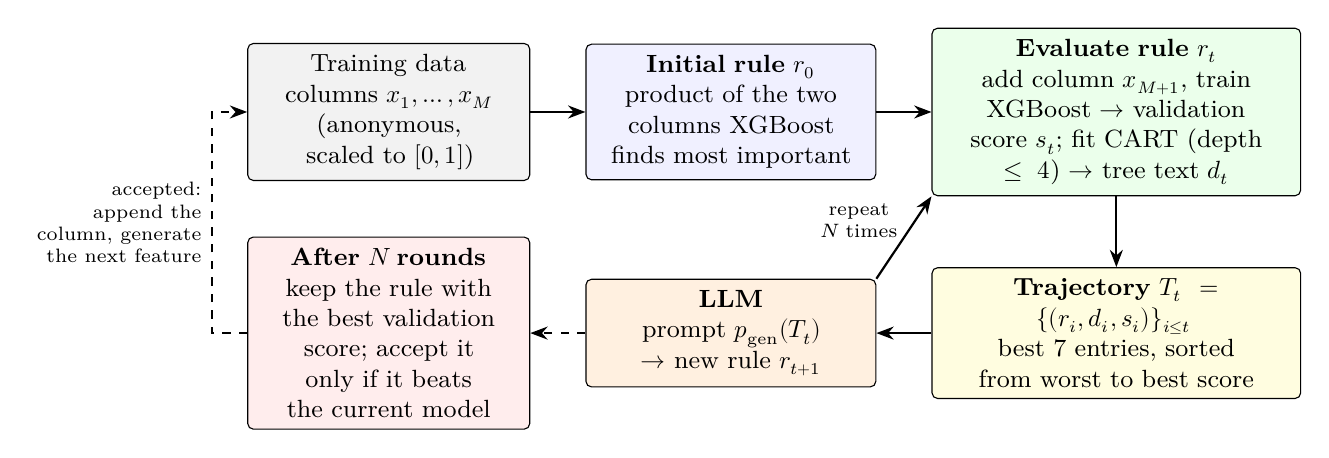
\begin{tikzpicture}[
  node distance=5mm and 7mm,
  box/.style={draw,rounded corners=2pt,align=center,font=\small,inner sep=4pt,fill=#1},
  box/.default=white,
  arr/.style={-{Stealth[length=2.2mm]},thick}]
\node[box=black!5,text width=3.3cm] (data) {Training data\\ columns $x_1,\dots,x_M$ (anonymous, scaled to $[0,1]$)};
\node[box=blue!6,text width=3.4cm,right=of data] (init) {\textbf{Initial rule $r_0$}\\ product of the two columns XGBoost finds most important};
\node[box=green!8,text width=4.4cm,right=of init] (eval) {\textbf{Evaluate rule $r_t$}\\ add column $x_{M+1}$, train XGBoost $\rightarrow$ validation score $s_t$; fit CART (depth $\le 4$) $\rightarrow$ tree text $d_t$};
\node[box=yellow!12,text width=4.4cm,below=9mm of eval] (traj) {\textbf{Trajectory} $T_t=\{(r_i,d_i,s_i)\}_{i\le t}$\\ best 7 entries, sorted from worst to best score};
\node[box=orange!12,text width=3.4cm,left=of traj] (llm) {\textbf{LLM}\\ prompt $p_{\text{gen}}(T_t)$ $\rightarrow$ new rule $r_{t+1}$};
\node[box=red!7,text width=3.3cm,left=of llm] (sel) {\textbf{After $N$ rounds}\\ keep the rule with the best validation score; accept it only if it beats the current model};
\draw[arr] (data) -- (init);
\draw[arr] (init) -- (eval);
\draw[arr] (eval) -- (traj);
\draw[arr] (traj) -- (llm);
\draw[arr] (llm.north east) -- node[pos=0.45,above left,font=\scriptsize,align=center,inner sep=1pt]{repeat\\ $N$ times} (eval.south west);
\draw[arr,dashed] (llm) -- (sel);
\draw[arr,dashed] (sel.west) -- ++(-0.45,0) |- node[pos=0.25,left,font=\scriptsize,align=right]{accepted:\\ append the\\ column, generate\\ the next feature} (data.west);
\end{tikzpicture}
\caption{The OCTree optimization loop in the context-agnostic setting (our drawing, after Figure 1 of
Nam et al., 2024). Test data is never used inside the loop.}
\label{fig:loop}
\end{figure}

\paragraph{Step 0: baseline.} The prediction model is trained on the original columns. Its
validation score is the reference that any new feature must beat.

\paragraph{Step 1: column name and initial rule.} When column names are meaningful
(\emph{context-aware} setting), the LLM first proposes a name for a useful new column (for example
``Trading Volume'' for stock prices) with prompt $p_{\text{col}}$, then an initial rule $r_0$ for
computing it with prompt $p_{\text{init}}$. In the \emph{context-agnostic} setting, which we
reproduce, there are no names to reason about: categorical columns are ordinal-encoded, all columns
are min-max scaled and renamed $x_1,\dots,x_M$, and the initial rule is simply the product of the two
columns with the highest XGBoost importance, e.g.\ $x_9=x_4\times x_1$.

\paragraph{Step 2: evaluation and decision tree reasoning.} For a rule $r_t$, the new column is
computed for every row, the model is retrained on the augmented training set and its validation
accuracy $s_t$ is recorded. In addition, a CART decision tree of maximum depth 4 is fitted to the
augmented training data and written out as nested if/else text $d_t$. The tree shows which columns
and thresholds separate the classes, and in particular whether, and at which level, the new column
is used. This is the ``decision tree reasoning'': information about the data learned from the whole
training set, expressed in a form an LLM can read.

\paragraph{Step 3: proposing a better rule.} The rules tried so far, with their trees and scores,
form a trajectory $T_t$. The LLM receives prompt $p_{\text{gen}}(T_t)$, which lists the entries
ordered by score so that the best ones come last (LLMs tend to build on what appears last in a list)
and asks for a new rule that is different from all previous ones and scores higher. The new rule is
evaluated as in Step 2 and appended to the trajectory. In the released code, the prompt shows the
seven best entries, the score is the validation accuracy multiplied by 10,000, and the prompt asks
for a rule in square brackets, using NumPy functions but avoiding unguarded division and logarithms.

\paragraph{Step 4: selection and further features.} After a fixed number of rounds (50 in the
paper) the rule with the highest validation score is selected. The column it produces is added to
the data, and the procedure starts again to generate another column on top of it. New columns are
added in sequence until the validation score no longer improves.

Algorithm~\ref{alg:octree} gives the same procedure as pseudocode.

\begin{algorithm}[H]
\caption{OCTree, context-agnostic setting (one dataset split)}\label{alg:octree}
\begin{algorithmic}[1]
\State $X \gets$ original columns; $s^{\star}\gets \text{ValScore}(X)$ \Comment{Step 0}
\Repeat
  \State $r_0 \gets x_a\times x_b$ for the two most important columns of $X$ \Comment{Step 1}
  \State $T\gets\{(r_0,\ \text{CART}(X\oplus r_0),\ \text{ValScore}(X\oplus r_0))\}$ \Comment{Step 2}
  \For{$t=0,\dots,N-1$}
    \State $r_{t+1}\gets \text{LLM}(p_{\text{gen}}(T))$ \Comment{Step 3}
    \State $T\gets T\cup\{(r_{t+1},\ \text{CART}(X\oplus r_{t+1}),\ \text{ValScore}(X\oplus r_{t+1}))\}$
  \EndFor
  \State $r^{\star}\gets$ rule in $T$ with the highest validation score \Comment{Step 4}
  \State \textbf{if} ValScore$(X\oplus r^{\star})>s^{\star}$ \textbf{then} $X\gets X\oplus r^{\star}$; $s^{\star}\gets$ ValScore$(X)$ \textbf{else} stop
\Until{stopped}
\State \Return $X$ and the model trained on it; report its test error once
\end{algorithmic}
\end{algorithm}

\subsection{What is new about OCTree}
\begin{itemize}
  \item \textbf{No fixed search space.} Classical AutoFE methods such as AutoFeat and OpenFE apply a
        predefined list of operators. OCTree lets the LLM write any expression, including
        conditional rules and trigonometric functions.
  \item \textbf{Feedback beyond a score.} Earlier methods, including CAAFE, judge a candidate only by
        its validation score and discard it if it does not help. OCTree keeps a history of attempts
        and adds a description of a decision tree trained with each candidate, so the LLM can see
        \emph{how} a feature was used, not only how well it scored.
  \item \textbf{Works without column descriptions.} Because the loop learns from feedback, it can
        be applied to anonymized data, which CAAFE cannot.
  \item \textbf{Model-agnostic features.} A feature optimized with XGBoost is an ordinary column, so
        it can also be given to other models (the paper shows gains for MLPs).
\end{itemize}

\subsection{Datasets and evaluation in the paper}
The paper evaluates on six datasets with column descriptions (e.g.\ Disease, Clinical Trial, Tesla
Stock) and on the 19 classification datasets of the Grinsztajn et al.\ (2022) benchmark without
descriptions, including electricity. Every dataset is split at random into 60\% training, 20\%
validation and 20\% test data, three times with different seeds. Classification is measured by test
error rate (\%), regression by mean absolute error, and results are reported as mean $\pm$ standard
deviation over the three splits, with the relative error reduction from the baseline in brackets.
The baseline models (XGBoost, an MLP and HyperFast) are tuned with 400 Optuna trials per split. The
main rule generator is a 7B Llama 2 model fine-tuned on the UltraChat dialogue data; GPT-4o is also
used in the context-aware experiments.

\subsection{Main findings of the paper}
\begin{itemize}
  \item On the 19 datasets without descriptions, OCTree lowers the XGBoost and MLP errors by about
        5\% on average (relative). The largest XGBoost gain is on electricity
        (Table~\ref{tab:paper}).
  \item With descriptions, OCTree beats CAAFE: average relative error reductions of 5.2\% (GPT-4o)
        and 2.9\% (Llama 2) against 1.7\% for CAAFE with GPT-4o.
  \item Removing the decision tree from the feedback still improves on the baseline, but less
        (Table~\ref{tab:paper}).
  \item Features found with XGBoost also improve MLP and HyperFast models.
\end{itemize}

\begin{table}[H]
\centering
\caption{Results reported by Nam et al.\ (2024) for XGBoost on electricity, the targets of our
reproduction. Test error (\%), mean $\pm$ standard deviation over three splits; relative error
reduction from the baseline in brackets.}
\label{tab:paper}
\begin{tabular}{@{}llr@{}}
\toprule
Setting & Source in the paper & Test error (\%) \\
\midrule
XGBoost on the original columns & Table 3 & $8.32\pm0.0$ \\
OCTree, scores and decision trees as feedback & Tables 3 and 6 & $6.65\pm0.1$ (20.1\%) \\
OCTree, scores only (no decision tree) & Table 6 & $6.89\pm0.6$ (17.2\%) \\
\bottomrule
\end{tabular}
\end{table}

% ======================================================================
\section{Implementation Details}\label{sec:impl}

\subsection{Environment and dependencies}
\begin{table}[H]
\centering
\caption{Computing environment.}
\label{tab:env}
\begin{tabularx}{\linewidth}{@{}lX@{}}
\toprule
Component & Used in this project \\
\midrule
Hardware & Google Colab, NVIDIA T4 GPU (XGBoost training) \\
Language & Python 3.13 (Colab) \\
Libraries & XGBoost 3.4.1, scikit-learn 1.6.1 (Pedregosa et al., 2011), NumPy 2.4.6, pandas 2.2.3, Matplotlib 3.10.0, \code{openai} 2.54.0 (API client), Streamlit \\
Rule-generating LLM & Gemini 3.5 Flash-Lite (\code{gemini-3.5-flash-lite}), Google AI Studio free tier, called through its OpenAI-compatible endpoint; temperature 1.0, top-$p$ 0.95 \\
Prediction model & XGBoost classifier, \code{tree\_method="hist"}, GPU \\
Feedback model & scikit-learn \code{DecisionTreeClassifier} (CART) \\
\bottomrule
\end{tabularx}
\end{table}

\subsection{Code structure}
The method code is in one module, \code{octree\_core.py}, organized in the order the method runs. The
notebook \code{OCTree\_Reproduction\_and\_Experiments.ipynb} calls it step by step, and four small
scripts provide the training, evaluation, inference and deployment entry points required by the
brief (Table~\ref{tab:files}).

\begin{table}[H]
\centering
\caption{Files in the submitted code.}
\label{tab:files}
\begin{tabularx}{\linewidth}{@{}lY@{}}
\toprule
File & Purpose \\
\midrule
\code{octree\_core.py} & Data loading and splits, XGBoost evaluation, safe rule evaluation, CART-to-text, prompt, LLM back-ends, optimization loop, experiments, final model and inference \\
\code{OCTree\_Reproduction\_and\_Experiments.ipynb} & Runs the reproduction, ablation, both experiments and the final model; produces all tables and figures \\
\code{train.py} & Training: runs OCTree from the command line and optionally saves the final model \\
\code{evaluate.py} & Evaluation: summarizes saved runs and compares them with the paper; with \code{--model}, scores the saved model (accuracy, precision, recall, F1, confusion matrix) \\
\code{predict.py} & Inference from the command line (one row or a CSV file) \\
\code{Deliverable\_2\_Electricity\_EDA\_and\_Preprocessing.ipynb} & Exploratory analysis and preprocessing (Section~\ref{sec:data}) \\
\code{sample\_input.csv} & Ten real test rows for trying the application's CSV upload \\
\code{app.py} & Deployment: Streamlit web application \\
\code{requirements.txt}, \code{README.md} & Dependencies; setup, experiment and launch instructions \\
\bottomrule
\end{tabularx}
\end{table}

\subsection{How each step is implemented}
\begin{enumerate}[label=\arabic*),leftmargin=*,itemsep=3pt]
\item \textbf{Data (\code{prepare\_data}, \code{load\_split})}\newline Downloads OpenML 44156 once, encodes the day
  code as an integer, draws a random permutation with seed 0, 1 or 2, splits it 60/20/20 and min-max
  scales every column with the training minimum and maximum. The scaling values are stored so that
  raw inputs can be transformed in the same way at inference time.
\item \textbf{Baseline and evaluation (\code{fit\_and\_score})}\newline Trains XGBoost with the authors' tuned
  hyperparameters for the split and returns training, validation and test accuracy. Only the
  validation accuracy is used for any decision.
\item \textbf{Rules (\code{extract\_rule}, \code{compile\_rule}, \code{apply\_rule})}\newline Reads the rule from the
  LLM's answer (\code{x9 = [ ... ]}, or a bare \code{[ ... ]}), checks that it contains only
  arithmetic, comparisons, the column names and a fixed list of NumPy and math functions, and
  evaluates it row by row. Rules that fail, return infinity or NaN, or repeat an earlier rule are
  rejected and the LLM is asked again. Each new column is min-max scaled with its training minimum
  and maximum, as in the authors' code.
\item \textbf{Initial rule (\code{initial\_rule})}\newline Fits default XGBoost models of depth 1 to 11, keeps the
  one with the best validation accuracy and multiplies its two most important columns.
\item \textbf{Decision tree reasoning (\code{fit\_cart}, \code{tree\_to\_text})}\newline Fits CART trees of depth 1
  to 4, keeps the best on validation data and writes it as if/else text with the authors' function.
\item \textbf{Prompt (\code{build\_prompt})}\newline The authors' prompt text, unchanged: the seven best rules so far
  from worst to best, each with its tree and its score (validation accuracy $\times$ 10,000). With
  \code{use\_tree=False} every mention of decision trees is removed, which gives the score-only
  ablation.
\item \textbf{LLM (\code{ChatLLM})}\newline Sends the prompt as a single user message and returns the text. It waits
  between calls, respects the provider's rate limits and records the number of calls, tokens and
  time.
\item \textbf{Optimization loop (\code{run\_octree})}\newline Steps 0--4 of Section~\ref{sec:method}: 50 proposals
  per feature, the best rule by validation accuracy (ties broken by lower training accuracy, as in
  the authors' code), accepted only if it improves validation accuracy, at most two generated
  features. The full state is written to \code{runs/<run>/seed<k>.json} after every step, so a run
  interrupted by a rate limit or a Colab disconnect resumes where it stopped.
\item \textbf{Final model (\code{train\_final\_model}, \code{predict})}\newline Retrains XGBoost on split 0 with the
  accepted features and saves the model and a pipeline description (scaling values and rules) for
  the application.
\end{enumerate}

\subsection{Code attribution}
The official implementation (\url{https://github.com/jaehyun513/OCTree}, files
\code{ours/train\_xg.py}, \code{ours/utils\_xg.py} and \code{ours/params.py}) was used as a
reference. Every function in \code{octree\_core.py} is labelled in the source as reused, adapted or
ours. Table~\ref{tab:attr} summarizes the labels.

\begin{table}[H]
\centering
\caption{Origin of each component.}
\label{tab:attr}
\begin{tabularx}{\linewidth}{@{}L{4.6cm}L{1.6cm}Y@{}}
\toprule
Component & Status & Detail \\
\midrule
Prompt text (\code{build\_prompt}) & Reused & Authors' \code{gen\_prompt}, wording unchanged; we added the option to leave out the trees \\
Tree as text (\code{tree\_to\_text}) & Reused & Authors' \code{tree\_to\_code} \\
Tuned XGBoost hyperparameters & Reused & Authors' published values for electricity, splits 0--2 \\
Rule-matching regular expression & Reused & Extended to handle answers without \code{x9 =} and model ``thinking'' text \\
Evaluation, CART selection, initial rule, optimization loop & Adapted & Same logic as the authors' \code{evaluate}, \code{get\_cart} and \code{train\_xg.py}, rewritten \\
Local Llama 2 back-end (\code{HFLocalLLM}) & Adapted & Authors' \code{load\_model} and \code{use\_api}; included but not used for our results \\
Data preparation & Ours & From our preprocessing notebook (Deliverable 2) \\
Safe rule evaluation & Ours & Replaces \code{exec()} of LLM-written code \\
API LLM back-end, rate-limit handling, resuming & Ours & Replaces the local GPU model \\
Hand-made features and data-size experiment & Ours & Section~\ref{sec:exp} \\
Final model, inference, \code{train.py}, \code{evaluate.py}, \code{predict.py}, \code{app.py} & Ours & Sections~\ref{sec:impl} and~\ref{sec:deploy} \\
\bottomrule
\end{tabularx}
\end{table}

\textbf{Results:} All numbers labelled ``ours'' in this report were produced by our runs of the
submitted code; numbers labelled ``paper'' are copied from Nam et al.\ (2024).

\textbf{Use of AI assistance:} An AI assistant (Claude, Anthropic) was used to help review and debug
the code, set up the Colab and LLM workflow, and edit parts of this report. The experiments were run
by the team, and all reported results come from those runs.

\subsection{Changes made to make the method feasible}
\begin{table}[H]
\centering
\caption{Differences from the paper and the released code, and the reason for each.}
\label{tab:changes}
\begin{tabularx}{\linewidth}{@{}L{4.3cm}L{4.7cm}Y@{}}
\toprule
Paper / original code & This project & Reason \\
\midrule
Fine-tuned Llama 2 7B on a local GPU & Gemini 3.5 Flash-Lite through a free API & No dedicated GPU; Colab's T4 is needed for XGBoost, and with depth-4 trees our prompts averaged about 2,300 tokens, close to the 4,096-token context of Llama 2 \\
19 + 6 datasets, three prediction models & Electricity, XGBoost only & Course scope \\
400 Optuna trials per split to tune XGBoost & Authors' published tuned values reused & Removes the tuning cost; same model as the paper \\
Features added until validation stops improving (electricity: up to $x_{12}$) & Same rule, capped at two features ($x_9$, $x_{10}$) & LLM call budget on a free tier (about 100 calls per split and run) \\
LLM output executed with \code{exec()} & Checked and evaluated with a restricted set of maths functions & Safety \\
CART depths 1--3 in the code, ``maximum depth of 4'' in the paper & Depths 1--4 & Follows the paper's text \\
A repeated rule is evaluated again & Rejected; a new rule is requested & The paper asks for rules not already in the trajectory \\
A rule giving inf/NaN is recorded, then retried & Rejected before being recorded & Keeps the trajectory clean \\
Answers of at most 256 new tokens & Answers of up to 4,096 tokens & Gemini sometimes writes its reasoning before the rule; a short limit cut the rule off \\
\bottomrule
\end{tabularx}
\end{table}

\subsection{Safeguards and reproducibility}
\begin{itemize}
  \item The test set is never shown to the LLM and never used to choose a rule; it is evaluated
        only for reporting.
  \item Splits, XGBoost and CART use fixed seeds. The LLM samples with temperature 1.0, so a repeated
        run can propose different rules; the saved run files record every proposed rule, its tree and
        its scores, so every reported result can be traced.
  \item Each run file stores its settings and refuses to resume with different ones, so results
        from different configurations cannot be mixed.
  \item The pipeline was first tested end to end on a small
        configuration (one split, five proposals) before the full run.
\end{itemize}

% ======================================================================
\section{Dataset and Preprocessing}\label{sec:data}

The purpose of this analysis is to understand the electricity dataset before modelling. We examine
data quality, class balance, feature distributions and relationships with the target. Detailed
exploratory analysis uses only the training subset, while validation and test observations are
reserved for evaluation. This section is carried over from Deliverable 2, with the preprocessing
steps now summarized in Table~\ref{tab:prep}.

\subsection{Dataset description and data quality}

The Australian Electricity dataset (Harries, 1999) was obtained from OpenML, dataset ID 44156
(Vanschoren et al., 2014). It contains 38,474 half-hourly observations from the New South Wales (NSW)
electricity market, eight input features and a binary target labelled UP or DOWN. The target
describes the NSW electricity price relative to a moving average of the preceding 24 hours.

The inputs include normalized electricity prices, demand, scheduled interstate transfer and temporal
indicators. The numerical values supplied cannot be interpreted directly as prices in currency units
or demand in megawatts.

Our checks found no missing values or exact duplicate rows. This is the balanced, shuffled benchmark
version used by Nam et al.\ (2024). Following that study, the data was divided into training (60\%),
validation (20\%) and test (20\%) sets using random splits over three seeds.

\begin{table}[H]
\centering
\caption{Dataset characteristics and split sizes (the same for each seed).}
\label{tab:dataset}
\begin{tabular}{@{}ll@{}}
\toprule
Dataset property & Value \\
\midrule
OpenML dataset ID & 44156 \\
Total observations & 38,474 \\
Original input features & 8 \\
Target classes & UP and DOWN \\
Missing entries & 0 \\
Exact duplicate rows & 0 \\
Training observations & 23,084 \\
Validation observations & 7,695 \\
Test observations & 7,695 \\
\bottomrule
\end{tabular}
\end{table}

\subsection{Example records}

Table~\ref{tab:examples} shows five example observations before our encoding and min-max scaling
steps. The numerical values are already normalized by the dataset source. Only selected columns are
displayed to keep the table readable.

\begin{table}[H]
\centering
\caption{Selected columns from the first five source observations, rounded to four decimal places.}
\label{tab:examples}
\begin{tabular}{@{}rrrrrl@{}}
\toprule
Period & NSW price & NSW demand & Victoria demand & Transfer & Class \\
\midrule
0.9574 & 0.0686 & 0.5683 & 0.4565 & 0.6447 & DOWN \\
0.2340 & 0.0337 & 0.3371 & 0.3296 & 0.8469 & DOWN \\
0.2553 & 0.0592 & 0.1858 & 0.4229 & 0.4149 & DOWN \\
0.5319 & 0.0876 & 0.5396 & 0.6378 & 0.4917 & DOWN \\
0.0851 & 0.0270 & 0.1651 & 0.2659 & 0.7482 & DOWN \\
\bottomrule
\end{tabular}
\end{table}

\subsection{Target-class distribution}

The training subset contains 11,503 DOWN observations (49.83\%) and 11,581 UP observations (50.17\%)
(Figure~\ref{fig:class}). The two classes are almost exactly balanced. Always predicting UP would
achieve 50.17\% training accuracy, providing a simple reference for model evaluation.

\begin{figure}[H]
\centering
\includegraphics[width=0.62\linewidth]{media/image2.png}
\caption{UP and DOWN class counts in the training subset.}
\label{fig:class}
\end{figure}

\subsection{Numerical feature distributions}

The numerical features have different distributions despite being supplied on normalized scales
(Figure~\ref{fig:hist}). Normalization changes their scale but does not remove skewness, repeated
values or unusual observations. Box plots were also examined in the notebook. Observations outside
their whiskers were retained because statistical unusualness alone does not establish a data error.

\begin{figure}[H]
\centering
\includegraphics[width=0.9\linewidth,height=0.36\textheight,keepaspectratio]{media/image3.png}
\caption{Numerical feature distributions in the training subset. All measurements retain their
supplied normalized scales.}
\label{fig:hist}
\end{figure}

\subsection{Feature differences between UP and DOWN}

\begin{table}[H]
\centering
\caption{Average normalized measurements by target class in the training subset.}
\label{tab:means}
\begin{tabular}{@{}lrr@{}}
\toprule
Mean normalized feature value & DOWN & UP \\
\midrule
NSW price & 0.0447 & 0.0763 \\
NSW demand & 0.3792 & 0.4899 \\
Victoria price & 0.0028 & 0.0042 \\
Victoria demand & 0.3985 & 0.4556 \\
Scheduled transfer & 0.5162 & 0.4790 \\
\bottomrule
\end{tabular}
\end{table}

UP observations have higher average NSW price and demand than DOWN observations
(Table~\ref{tab:means}). Victoria price and demand also have higher averages in the UP group, while
scheduled transfer has a lower average. These differences suggest potentially useful information for
classification. However, the grouped box plots in the notebook show overlap between classes, so
group averages do not provide a perfect classification rule.

\subsection{Correlation analysis}

NSW price has the strongest positive Pearson correlation with the UP target among the numerical
features examined (0.362), followed by NSW demand (0.342). Scheduled transfer has a negative
correlation of $-0.123$ (Figure~\ref{fig:corr}). These results describe linear associations within
the training subset. Correlation does not establish causation, and weak linear correlation does not
rule out useful nonlinear relationships or interactions, which is exactly what generated features
aim to capture. NSW price is also closely connected to the target definition, so its association
with the target should not be presented as evidence of forecasting a future price.

\begin{figure}[H]
\centering
\includegraphics[width=0.75\linewidth,height=0.38\textheight,keepaspectratio]{media/image4.png}
\caption{Pearson correlations among numerical features and the binary target in the training subset.
UP is encoded as 1 and DOWN as 0.}
\label{fig:corr}
\end{figure}

\subsection{Day-of-week patterns}

The percentage of UP observations varies across day-of-week codes. It is 55.66\% for code 0 and
46.84\% for code 5 (Figure~\ref{fig:day}). This suggests that day-of-week information may contribute
to classification. These differences describe the training sample and do not establish that the day
itself causes price changes.

\begin{figure}[H]
\centering
\includegraphics[width=0.7\linewidth,height=0.32\textheight,keepaspectratio]{media/image5.png}
\caption{UP and DOWN percentages calculated separately within each day-of-week code.}
\label{fig:day}
\end{figure}

\subsection{Patterns across the observation sequence}

Rolling averages were used to examine demand and UP-label frequency over time
(Figure~\ref{fig:time}). As the dataset is shuffled, time order was rebuilt from the date and period
columns, and daily averages were smoothed over seven observed date values. The rebuilt time order is
approximate: a few date values cover two day-of-week codes, and some observations were removed when
the classes were balanced, so exact calendar continuity cannot be confirmed. Changes in demand or
label frequency alone do not prove concept drift in the relationship between inputs and target.

\begin{figure}[H]
\centering
\includegraphics[width=0.9\linewidth,height=0.34\textheight,keepaspectratio]{media/image6.png}
\caption{Rolling mean demand and UP-label proportion across the training data in time order, using a
seven-observed-date rolling window.}
\label{fig:time}
\end{figure}

\subsection{Preprocessing}

Table~\ref{tab:prep} lists every preprocessing step. The same code is used by the preprocessing
notebook, by \code{octree\_core.py} and, through the saved scaling values, by the deployed
application.

\begin{table}[H]
\centering
\caption{Preprocessing steps.}
\label{tab:prep}
\begin{tabularx}{\linewidth}{@{}L{3.6cm}Y@{}}
\toprule
Step & Decision \\
\midrule
Target & Both target columns excluded from the inputs; DOWN $=0$, UP $=1$; UP is the positive class \\
Missing values & Rows with missing values are removed (none were found) \\
Categorical feature & Day-of-week code ordinal-encoded as integers 0--6 \\
Splits & Random 60/20/20 split, repeated with seeds 0, 1 and 2, as in the paper \\
Scaling & Every column min-max scaled with the training minimum and maximum only; validation and test values may fall slightly outside $[0,1]$ \\
Anonymization & Columns renamed $x_1,\dots,x_8$ (date, day, period, NSW price, NSW demand, Victoria price, Victoria demand, transfer) so the LLM cannot use their meaning \\
Generated columns & Computed from the scaled columns and min-max scaled with their own training minimum and maximum \\
Verification & No missing or infinite values in any processed split \\
\bottomrule
\end{tabularx}
\end{table}

Typical image or text preprocessing such as resizing, augmentation or tokenization does not apply
to this tabular task. The closest equivalent in OCTree is the conversion of rules, trees and scores
into the text prompt described in Section~\ref{sec:method}.

\subsection{Evaluation metrics}

The classes are almost exactly balanced, so test error rate, the metric reported in the paper, is the
main measure; it equals one minus accuracy. As in the paper, results are given as mean $\pm$ standard
deviation over the three splits, with the relative error reduction
$100\times(\text{err}_{\text{baseline}}-\text{err})/\text{err}_{\text{baseline}}$. For the deployed
model we also report precision, recall, F1 for the UP class and a confusion matrix.

% ======================================================================
\section{Reproduction Results}\label{sec:repro}

\subsection{Baseline}
Table~\ref{tab:baseline} shows XGBoost with the authors' tuned hyperparameters on the original eight
columns. Our mean test error of $8.50\pm0.16\%$ is 0.18 percentage points above the paper's
$8.32\%$. The difference is smaller than the spread between our splits. Our three splits are
identical to the split files the authors published (the deployed model gives exactly the same test
error on their split-0 file), so the gap most likely comes from a newer XGBoost version and different
GPU hardware, which change the fitted trees slightly.

\begin{table}[H]
\centering
\caption{XGBoost on the original columns (ours), with the authors' tuned hyperparameters.}
\label{tab:baseline}
\begin{tabular}{@{}crrrr@{}}
\toprule
Split & Validation accuracy (\%) & Test accuracy (\%) & Test error (\%) & Training time (s) \\
\midrule
0 & 91.35 & 91.59 & 8.41 & 13.5 \\
1 & 91.40 & 91.63 & 8.37 & 9.0 \\
2 & 90.83 & 91.27 & 8.73 & 23.7 \\
\midrule
Mean $\pm$ std & & & $8.50\pm0.16$ & \\
Paper & & & $8.32\pm0.0$ & \\
\bottomrule
\end{tabular}
\end{table}

\subsection{OCTree}
OCTree ran with 50 proposals per feature and at most two generated features on each of the three
splits. On every split both generated features were accepted, and the test error fell on every
split (Table~\ref{tab:octree}).

\begin{table}[H]
\centering
\caption{OCTree with XGBoost on electricity: our results against the paper. Test error (\%); relative
error reduction from the baseline in brackets. ``Starting rule only'' adds just the initial rule
$x_9=x_4\times x_1$, before any LLM proposal.}
\label{tab:octree}
\begin{tabular}{@{}lcccc@{}}
\toprule
 & Baseline & Starting rule only & OCTree & Features kept \\
\midrule
Split 0 & 8.41 & 8.36 & 7.76 (7.7\%) & 2 \\
Split 1 & 8.37 & 8.36 & 7.52 (10.1\%) & 2 \\
Split 2 & 8.73 & 8.62 & 7.71 (11.8\%) & 2 \\
\midrule
\textbf{Ours}, mean $\pm$ std & $8.50\pm0.16$ & $8.44\pm0.12$ & \textbf{$7.66\pm0.10$} \textbf{(9.9\%)} & \\
Paper (Tables 3 and 6) & $8.32\pm0.0$ & --- & $6.65\pm0.1$ (20.1\%) & up to 4 \\
\bottomrule
\end{tabular}
\end{table}

\textbf{Reproduction verdict:} The paper's main claim holds in our setting: features generated by an
LLM from anonymous columns, guided by validation scores and decision trees, lower the XGBoost test
error on electricity, on all three splits and by much more than the spread between splits. The size
of the gain is about half of the paper's (9.9\% against 20.1\% relative reduction; 7.66\% against
6.65\% error). Section~\ref{sec:analysis} discusses the likely reasons.

Two checks show that the gain is real and comes from the LLM. First, the starting rule on its own
($x_4\times x_1$, chosen without any LLM) gives $8.44\%$, so almost all of the improvement to
$7.66\%$ comes from the rules the LLM proposed. Second, with 7,695 test rows and an error near
8.5\%, the standard error of a single test error is about
0.32 percentage points (the square root of $0.085\times0.915/7695$); the OCTree gain of 0.84 points is well
above this, and it appears on every split. Differences between methods smaller than about 0.3 points,
including the 0.18-point gap between our baseline and the paper's, should be treated as noise.

\textbf{Search behaviour:} Figure~\ref{fig:search} shows every proposed rule and the best validation
accuracy so far. Improvements arrive in a few steps rather than gradually, and most proposals score
below the best rule; where the LLM found a better rule, it did so after 11 to 46 proposals. On split 2
none of the 50 proposals for $x_9$ beat the initial rule $x_4\times x_1$, which was therefore kept; the
search for $x_{10}$ then raised validation accuracy from 90.94\% to 91.81\%.

\begin{figure}[H]
\centering
\includegraphics[width=\linewidth]{media/fig_search_progress.png}
\caption{Validation accuracy of every OCTree rule (grey) and the best so far with decision tree
feedback (blue) and without it (orange, the ablation of Section 6.3). Rules 0--50 search for $x_9$,
rules 51--101 for $x_{10}$ on top of the accepted $x_9$; the dotted line is XGBoost on the original
columns.}
\label{fig:search}
\end{figure}

\textbf{Accepted rules:} Table~\ref{tab:rules} lists the first accepted rule on each split and its
meaning in terms of the real columns, which the LLM never saw. All three contain the product of NSW
price and date ($x_4\times x_1$), the initial rule, and the rules on split 0 branch on
$x_4>0.07$, the first split of the decision tree shown in the prompt. The second rules are longer
combinations of the same ingredients and are listed in the run files.

\begin{table}[H]
\centering
\caption{First accepted rule ($x_9$) on each split. Columns: $x_1$ date, $x_2$ day, $x_3$ period, $x_4$
NSW price, $x_5$ NSW demand, $x_6$ Victoria price, $x_7$ Victoria demand, $x_8$ transfer (all scaled to
$[0,1]$).}
\label{tab:rules}
\begin{tabular}{@{}cp{7.4cm}p{6.2cm}@{}}
\toprule
Split & Rule & Meaning \\
\midrule
0 & \code{np.where(x4 > 0.07, x1*x3*x4 + np.sin(x6*x8)*(1 - x2), np.cos(x5*x7) + x1*x2*(1 - x4))} & In
the high-price regime: date $\times$ period $\times$ NSW price plus a Victoria-price$\times$transfer
term; otherwise a demand interaction plus date $\times$ day \\
1 & \code{x4*x1*(x3 + x5 + 1)*(np.abs(x1 - x5) + 1)*np.maximum(x2, x6)} & NSW price $\times$ date,
scaled up by period and NSW demand \\
2 & \code{x4*x1} & NSW price $\times$ date (initial rule) \\
\bottomrule
\end{tabular}
\end{table}

\textbf{Cost:} Table~\ref{tab:cost} summarizes the run. Training XGBoost took most of the time; the
LLM calls cost nothing on the free tier. About one answer in eight could not be used (for example, no rule could be read from it, or it
repeated an earlier rule), and the LLM was asked again.

\begin{table}[H]
\centering
\caption{Cost of the OCTree run (three splits, 50 proposals per feature, two features).}
\label{tab:cost}
\begin{tabular}{@{}lr@{}}
\toprule
Item & Value \\
\midrule
LLM calls (usable rules $+$ unusable answers) & 341 (300 $+$ 41) \\
LLM calls for the ablation run & 327 (300 $+$ 27) \\
Prompt / answer tokens & 795,732 / 31,942 \\
Time training XGBoost & 73.5 min \\
Time waiting for the LLM & 14.3 min \\
Time for CART trees and rule evaluation & 2.9 min \\
\bottomrule
\end{tabular}
\end{table}

\subsection{Ablation: scores only, without decision trees}
The ablation repeats the full run with the decision trees removed from the prompt, so the LLM sees
only rules and scores (Table 6 of the paper). Everything else is unchanged.

\begin{table}[H]
\centering
\caption{Ablation: OCTree with and without decision tree feedback. Test error (\%); relative
reduction from the baseline in brackets.}
\label{tab:ablation}
\begin{tabular}{@{}lccc@{}}
\toprule
 & Baseline & Scores only (no trees) & Scores and trees (OCTree) \\
\midrule
Split 0 & 8.41 & 7.68 & 7.76 \\
Split 1 & 8.37 & 7.37 & 7.52 \\
Split 2 & 8.73 & 8.07 & 7.71 \\
\midrule
\textbf{Ours}, mean $\pm$ std & $8.50\pm0.16$ & $7.71\pm0.29$ (9.4\%) & $7.66\pm0.10$ (9.9\%) \\
Paper (Table 6) & $8.32\pm0.0$ & $6.89\pm0.6$ (17.2\%) & $6.65\pm0.1$ (20.1\%) \\
\bottomrule
\end{tabular}
\end{table}

Both versions improve on the baseline on every split. On average the full method is slightly
better (7.66\% against 7.71\%), but the difference of 0.05 points is far below the test-set noise of
about 0.3 points, so the means do not show that the trees help. What differs clearly is the spread:
with trees the three splits end within 0.24 points of each other ($\pm0.10$); without them the
results range from 7.37\% to 8.07\% ($\pm0.29$), and on split 2 the score-only run gained much less.
The paper shows the same pattern, a slightly lower mean and a much smaller spread with trees ($\pm0.1$
against $\pm0.6$). Figure~\ref{fig:search} shows that without trees the LLM sometimes reached higher
validation accuracy (splits 0 and 1) and sometimes much lower (split 2).

% ======================================================================
\section{Additional Experiments}\label{sec:exp}

Both experiments use the same splits and the same XGBoost settings as the reproduction, and need no
extra LLM calls.

\subsection{Experiment 1: hand-made features vs OCTree (baseline comparison)}
\textbf{Question:} OCTree generates features without knowing what $x_1,\dots,x_8$ mean. A person who
knows the columns can design features from that knowledge. Do such hand-made features match or beat
the features of an LLM that sees only anonymous columns and feedback?

\textbf{Setup:} We designed seven features from the meaning of the columns
(Table~\ref{tab:manual}). For a fair comparison:
\begin{itemize}
  \item each hand-made feature uses only the values in the same row, like OCTree's rules. Features
        that look at earlier half-hours (such as a moving average of the price) are excluded,
        because OCTree cannot build them and because rows removed during class balancing break the
        sequence;
  \item hand-made features are selected with exactly OCTree's rule: each candidate is tried as
        $x_9$, the best on validation data is kept only if it beats the original columns, and the
        rest are tried as $x_{10}$ on top of it, up to two features;
  \item we also report all seven added at once without selection.
\end{itemize}

\begin{table}[H]
\centering
\caption{Hand-made candidate features ($x_1$ date, $x_2$ day, $x_3$ period, $x_4$ NSW price, $x_5$
NSW demand, $x_6$ Victoria price, $x_7$ Victoria demand, $x_8$ transfer).}
\label{tab:manual}
\begin{tabularx}{\linewidth}{@{}lL{4.1cm}Y@{}}
\toprule
Feature & Rule & Reason \\
\midrule
price\_gap & $x_4-x_6$ & NSW price above Victoria's suggests a price movement \\
demand\_gap & $x_5-x_7$ & Relative pressure on the two markets \\
price\_x\_demand & $x_4\cdot x_5$ & High price under high demand signals a tight market \\
period\_sin & $\sin(2\pi x_3)$ & Time of day as a circle (23:30 next to 00:00), first coordinate \\
period\_cos & $\cos(2\pi x_3)$ & Time of day as a circle, second coordinate \\
peak\_hours & $1$ if $14/47\le x_3<44/47$ else $0$ & About 07:00--22:00, when demand and prices peak \\
transfer\_x\_price\_gap & $x_8\,(x_4-x_6)$ & Interstate flow weighted by the price gap \\
\bottomrule
\end{tabularx}
\end{table}

\textbf{Results:} Table~\ref{tab:exp1} and Figure~\ref{fig:exp1} give the test errors. On splits 0
and 1 no hand-made feature improved validation accuracy, so none was kept; on split 2,
\code{price\_gap} and \code{peak\_hours} were kept and lowered the error from 8.73\% to 8.53\%.
Adding all seven without selection made every split worse.

\begin{table}[H]
\centering
\caption{Hand-made features against OCTree. Test error (\%) per split, and mean $\pm$ std with the
relative reduction from the original columns.}
\label{tab:exp1}
\begin{tabular}{@{}lcccc@{}}
\toprule
 & Original columns & All 7 hand-made & Selected hand-made & OCTree \\
\midrule
Split 0 & 8.41 & 8.98 & 8.41 (none kept) & 7.76 \\
Split 1 & 8.37 & 8.90 & 8.37 (none kept) & 7.52 \\
Split 2 & 8.73 & 9.25 & 8.53 (2 kept) & 7.71 \\
\midrule
Mean $\pm$ std & $8.50\pm0.16$ & $9.04\pm0.15$ ($-6.4\%$) & $8.44\pm0.07$ (0.8\%) & \textbf{$7.66\pm0.10$} (9.9\%) \\
\bottomrule
\end{tabular}
\end{table}

\begin{figure}[H]
\centering
\includegraphics[width=0.85\linewidth]{media/fig_handmade_vs_octree.png}
\caption{Test error of each feature set, mean $\pm$ standard deviation over the three splits.}
\label{fig:exp1}
\end{figure}

\textbf{Answer:} No. With the same selection rule and the same model, OCTree's features beat the
hand-made ones on all three splits (7.66\% against 8.44\%), even though the LLM never knew what the
columns meant. The intuitive features describe relationships XGBoost already learns from the
original columns (a price gap is two splits away), whereas OCTree's rules combine four or five
columns with non-linear terms, which is harder for trees to approximate. Adding many features
without validation-based selection hurts, which supports OCTree's practice of accepting a feature only
when it improves the validation score.

\subsection{Experiment 2: training-set size (data-size experiment)}
\textbf{Question:} A tree splits on one column at a time, so it needs many examples to approximate a
relationship between columns. A generated column provides that relationship directly. Do generated
features therefore help more when training data is scarce?

\textbf{Setup:} XGBoost is trained on 10\%, 25\%, 50\% and 100\% of the training rows (random nested
subsets with a fixed seed), with three inputs: the original columns, the original columns plus the
selected hand-made features, and the original columns plus OCTree's features. Validation and test
sets are always the full ones, so every result is measured on the same rows, and XGBoost keeps the
same tuned settings at every size. If the hypothesis holds, the error reduction from generated
features should be largest at the smallest training size.

\textbf{Scope:} OCTree's features were found with the full training set. The experiment therefore
asks whether a \emph{given} feature is more useful with less data, not whether OCTree would
\emph{find} as good a feature from less data, which would require a new search for each size.

\textbf{Results:} Table~\ref{tab:exp2} and Figure~\ref{fig:exp2} give the results.

\begin{table}[H]
\centering
\caption{Test error (\%, mean $\pm$ std over three splits) for each training-set size, and the
reduction from the original columns in percentage points (pp).}
\label{tab:exp2}
\begin{tabular}{@{}rrcccc@{}}
\toprule
Fraction & Rows & Original & Hand-made & OCTree & OCTree gain \\
\midrule
10\% & 2,308 & $17.21\pm0.58$ & $17.19\pm0.61$ & $17.10\pm0.53$ & 0.11 pp \\
25\% & 5,771 & $13.67\pm0.09$ & $13.68\pm0.08$ & $13.20\pm0.26$ & 0.46 pp \\
50\% & 11,542 & $11.13\pm0.30$ & $11.02\pm0.42$ & $10.64\pm0.33$ & 0.49 pp \\
100\% & 23,084 & $8.50\pm0.16$ & $8.43\pm0.07$ & $7.66\pm0.10$ & 0.84 pp \\
\bottomrule
\end{tabular}
\end{table}

\begin{figure}[H]
\centering
\includegraphics[width=\linewidth]{media/fig_data_size.png}
\caption{Left: test error against the number of training rows. Right: error reduction from the
generated features (positive = the features help); error bars are standard deviations over the three
splits.}
\label{fig:exp2}
\end{figure}

\textbf{Answer:} The hypothesis is rejected. OCTree's features help at every size, but the gain grows
with the amount of data, from 0.11 percentage points at 10\% (within the spread between splits) to
0.84 points with the full training set; in relative terms the reduction rises from 0.6\% to 9.9\%.
Three explanations fit this result. (1) The features were chosen to maximize validation accuracy for
a model trained on the full set, so they are best matched to that size. (2) The rules are complex,
conditional combinations of several columns; with few rows, XGBoost (whose deep trees were tuned
for the full set) cannot estimate reliably how to use them. (3) With little data the error is
dominated by variance, which an extra column does not reduce. The hand-made features stay close to
zero gain at every size, as in Experiment 1.

% ======================================================================
\section{Analysis and Discussion}\label{sec:analysis}
\subsection{Why our gain is smaller than the paper's}
Our reproduction confirms the direction of the paper's result but reaches about half the error
reduction. Four differences can explain the gap:
\begin{itemize}
  \item \textbf{Fewer features:} We stopped at two generated features; the authors' electricity run
        went up to $x_{12}$. On every split the second feature still improved validation accuracy,
        so further features would probably have lowered the error more.
  \item \textbf{A different LLM:} The paper uses Llama 2 7B fine-tuned for dialogue; we used Gemini 3.5
        Flash-Lite. The paper itself reports that results depend on the LLM (its Table 4), and our
        model repeated itself often: on split 1, most later proposals were small edits of one
        formula.
  \item \textbf{Different software:} The splits are the same as the authors', but our baseline error
        is 0.18 points higher (newer XGBoost, different GPU), so the starting points are not exactly
        identical.
  \item \textbf{Randomness:} A single LLM run per split; the paper's three-run spread on electricity
        is small ($\pm0.1$), but ours may differ.
\end{itemize}

\subsection{What the generated features capture}
The accepted rules share a common ingredient: the product of NSW price and date ($x_4\times x_1$),
the initial rule that the LLM then refined. NSW price is the input most strongly correlated with
the target (Section~\ref{sec:data}), and date lets the model separate price levels from different
periods, which matters because the target compares the price with its own recent average. The
threshold $x_4>0.07$ that many rules use sits between the class averages of the scaled NSW price: the
mean price is 0.045 for DOWN and 0.076 for UP (Table~\ref{tab:means}). The LLM most likely took this
boundary from the decision tree in the prompt, since nothing in the prompt describes the columns.

\subsection{Did the decision tree feedback help?}
There is direct evidence that the LLM reads the trees. On split 0, 46 of 50 proposals for $x_9$
branch on exactly $x_4>0.07$, the first split of the tree in every prompt, and on split 2, 41 of 50
proposals for $x_{10}$ do the same; on split 1 the LLM never used such a branch. The feedback is also
limited: the tree is fitted with depth at most 4, and only about a third of the trees (100 of 306)
used the new feature at all, so in most rounds the tree in the prompt looked almost the same as
before.

The ablation confirms that the threshold comes from the trees: without them, none of the 300
proposals used a branch on $x_4>0.07$ or $x_4>0.08$, and the rules were longer: in two search rounds the
average rule had about 350 characters, against at most about 230 in any round with trees. It does not show a clear gain in average test error
(Section 6.3); the benefit we observe is stability. With trees, the LLM's proposals stay anchored to
the structure of the data and every split improves by a similar amount; without them, the search
depends more on chance and can end far from the best result, as on split 2. With three splits and
one run per split this is suggestive rather than conclusive, but it agrees with the paper, whose
score-only variant also has a six times larger spread.

\subsection{What the experiments add}
The two experiments point the same way. Generated features help because they encode multi-column,
non-linear structure that a validation-guided search can find and a person would not think of;
features that reflect intuition about the columns did not help this model. The benefit appears when
the model has enough data to use such complex columns, and selection on validation data is
essential: adding features blindly made the model worse.

% ======================================================================
\section{Model Deployment}\label{sec:deploy}

\subsection{Inference pipeline}
The deployed system follows the pipeline \textbf{Input $\rightarrow$ Preprocessing $\rightarrow$
Trained model $\rightarrow$ Prediction $\rightarrow$ Output}:
\begin{enumerate}
  \item \textbf{Input:} eight values in the dataset's own scale, typed into a form or uploaded as a
        CSV file.
  \item \textbf{Preprocessing:} each value is min-max scaled with the training minimum and maximum
        saved in \code{model/pipeline.json}; the generated features are computed from the scaled
        values with the saved OCTree rules and scaled with their saved minimum and maximum.
  \item \textbf{Trained model:} the XGBoost model saved in \code{model/xgb\_model.json}.
  \item \textbf{Prediction and output:} the probability of UP and the label (UP if the probability
        is at least 0.5).
\end{enumerate}
The rules are stored as text in \code{pipeline.json}, so no LLM or internet connection is needed at
prediction time.

\subsection{How to start the application}
\begin{lstlisting}
pip install -r requirements.txt
streamlit run app.py          # opens http://localhost:8501
\end{lstlisting}
Dependencies: Python 3.10 or newer, \code{streamlit}, \code{xgboost}, \code{numpy}, \code{pandas},
\code{scikit-learn}. The folder \code{model/} produced by the notebook (Section 8) must be next to
\code{app.py}.

\subsection{The application}
The Streamlit application (\code{app.py}) has three tabs. \textbf{Single prediction} groups the eight
inputs into time (date, day, half-hour slot) and market values (prices, demand, transfer); a button
loads a real test example so that the prediction can be compared with its true label. The result is
shown as a large UP or DOWN card with the probabilities of both classes, and an expandable table
shows each preprocessing step: the raw value, the scaled value given to the model and the generated
features computed from them. \textbf{CSV file} predicts every row of an uploaded file and offers the
result for download. \textbf{How it works} lists the accepted rules with their meaning in terms of
the real column names, and the model's test metrics. The sidebar shows the model's test error and
the generated features at all times.

\subsection{Input and output format}
\begin{table}[H]
\centering
\caption{Input format: eight values in this order, on the dataset's normalised scale.}
\label{tab:io}
\begin{tabular}{@{}lll@{}}
\toprule
Column & Meaning & Range \\
\midrule
date & Date & 0--1 \\
day & Day-of-week code & 0--6 \\
period & Half-hour of the day (slot $\div$ 47) & 0--1 \\
nswprice, nswdemand & NSW price and demand & 0--1 \\
vicprice, vicdemand & Victoria price and demand & 0--1 \\
transfer & Scheduled transfer between the states & 0--1 \\
\bottomrule
\end{tabular}
\end{table}
\textbf{Output:} the label UP or DOWN (NSW price relative to its 24-hour moving average) and the
model's probability of UP. The CSV tab returns the uploaded file with two added columns,
\code{prediction} and \code{probability\_UP}, which can be downloaded.

\subsection{Example inference}
The final model is XGBoost trained on split 0 with the two rules OCTree accepted on that split. It
reaches a validation accuracy of 92.15\% and a test error of 7.76\%, the split-0 result of
Table~\ref{tab:octree}. One test example passed through the whole pipeline:
\begin{lstlisting}
Input     : date 0.89381, day 3, period 0.06383, nswprice 0.053381, nswdemand 0.463106,
            vicprice 0.003556, vicdemand 0.481875, transfer 0.528947
Prediction: DOWN  (probability of UP = 0.001)   true label: DOWN
\end{lstlisting}
Table~\ref{tab:deploymetrics} gives the metrics of the deployed model on the 7,695 test rows of split
0, computed by passing the raw test values through the same pipeline the application uses (notebook
Section 8.1, or \code{python evaluate.py --model model}). The test error of 7.76\% equals the result
in Table~\ref{tab:octree}, which confirms that the deployed pipeline reproduces the experiment. Errors
are balanced between the classes: 311 DOWN half-hours were predicted UP and 286 UP half-hours were
predicted DOWN.

\begin{table}[H]
\centering
\caption{Metrics of the deployed model on the split-0 test set (UP is the positive class).}
\label{tab:deploymetrics}
\begin{tabular}{@{}lr@{\hspace{2.5em}}lrr@{}}
\toprule
Metric & Value & Confusion matrix & Predicted DOWN & Predicted UP \\
\midrule
Accuracy & 92.24\% & True DOWN & 3,556 & 311 \\
Test error & 7.76\% & True UP & 286 & 3,542 \\
Precision (UP) & 91.93\% & & & \\
Recall (UP) & 92.53\% & & & \\
F1 (UP) & 92.23\% & & & \\
\bottomrule
\end{tabular}
\end{table}

\subsection{Application screenshots}
Figures~\ref{fig:app1}--\ref{fig:app3} show the application running with the final model.

\begin{figure}[H]
\centering
\includegraphics[width=0.92\linewidth]{media/app_screenshot_1.png}
\caption{The application at start-up: input form, and the model's test error (7.76\%) and the two
generated features in the sidebar.}
\label{fig:app1}
\end{figure}

\begin{figure}[H]
\centering
\includegraphics[width=0.92\linewidth]{media/app_screenshot_2.png}
\caption{A prediction for a real test example, with the preprocessing steps shown.}
\label{fig:app2}
\end{figure}

\begin{figure}[H]
\centering
\includegraphics[width=0.92\linewidth]{media/app_screenshot_3.png}
\caption{Batch prediction from an uploaded CSV file (\code{sample\_input.csv}).}
\label{fig:app3}
\end{figure}

% ======================================================================
\section{Limitations}\label{sec:limits}
\begin{itemize}
  \item \textbf{Different LLM:} We used Gemini 3.5 Flash-Lite instead of the authors' fine-tuned
        Llama 2 7B. The paper shows that the choice of LLM changes the result (its Table 4), so our
        numbers measure OCTree with a different rule generator, not an exact replication.
  \item \textbf{Feature cap:} At most two generated features, while the authors' electricity run
        reached four.
  \item \textbf{One dataset and one model:} Only electricity and XGBoost; the paper's claims about
        MLPs, HyperFast and the other 18 datasets were not tested.
  \item \textbf{Three splits:} Means over three splits give only a rough estimate of variability, and
        LLM sampling adds randomness that a single run per split does not capture.
  \item \textbf{Contemporaneous task:} The current NSW price is an input, so the task classifies the
        present price relative to its moving average; it is not a forecast of future prices.
  \item \textbf{Approximate time order:} The benchmark version is shuffled and class-balanced, so
        temporal dependence between rows is ignored by the random splits.
\end{itemize}
\begin{itemize}
  \item \textbf{Test-set noise:} With 7,695 test rows, a difference of about 0.3 percentage points can
        arise by chance, so small differences between feature sets are not conclusive.
  \item \textbf{Hardware dependence:} XGBoost gives slightly different results on CPU and GPU
        (differences of about 0.1 points in our tests), which can change which candidate feature is
        selected when candidates are close.
  \item \textbf{Free-tier limits:} The free Gemini tier allowed 500 requests per day, so the ablation
        had to be split over two days; the run resumed from its saved state without any change.
  \item \textbf{Unusable answers:} About 12\% of LLM answers could not be used, which costs calls
        on a rate-limited API.
  \item \textbf{Repetitive proposals:} On some splits the LLM produced many near-identical variants of
        one rule, which limits exploration.
  \item \textbf{Interpretability:} The accepted rules are long expressions that are hard to explain
        in terms of the market, even after mapping the columns back to their names.
\end{itemize}

% ======================================================================
\section{Conclusion}\label{sec:conclusion}
We re-implemented OCTree in its context-agnostic setting and reproduced it on the electricity
dataset with XGBoost, using a free API LLM in place of the authors' Llama 2 model. With two generated
features per split, the test error fell from $8.50\pm0.16\%$ to $7.66\pm0.10\%$ (9.9\% relative
reduction) on all three splits. Removing the decision trees from the feedback gave a similar
average ($7.71\%$) but results three times more spread between splits, the same pattern as in the
paper. This confirms the paper's main claim, that an LLM guided by validation
scores and decision trees can improve features without knowing what the columns mean, while the size
of the improvement is about half of the reported 20.1\%, most likely because we generated fewer
features with a different LLM.

Our two experiments add to this. Features designed by hand from the column meanings did not beat
OCTree's (8.44\% against 7.66\%), and adding them all without selection made the model worse. Contrary
to our expectation, the generated features helped more as the training set grew, not less. The
final model is deployed as a Streamlit application that takes eight raw values and returns UP or DOWN
with a probability, applying the generated features automatically.

Natural next steps are to let OCTree add features until validation stops improving, as in the
paper, to repeat the search with other LLMs, and to test whether the features transfer to other
models.

% ======================================================================
\clearpage
\section{References}\label{sec:refs}
\small
\raggedright
\setlength{\parskip}{4pt}
\setlength{\parindent}{-0.5in}
\setlength{\leftskip}{0.5in}

Arik, S. Ö., \& Pfister, T. (2021). TabNet: Attentive interpretable tabular learning.
\emph{Proceedings of the AAAI Conference on Artificial Intelligence, 35}(8), 6679--6687.

Bordt, S., Nori, H., Rodrigues, V., Nushi, B., \& Caruana, R. (2024). Elephants never forget:
Memorization and learning of tabular data in large language models. In \emph{Proceedings of the First
Conference on Language Modeling}.

Borisov, V., Seßler, K., Leemann, T., Pawelczyk, M., \& Kasneci, G. (2023). Language models are
realistic tabular data generators. In \emph{International Conference on Learning Representations}.

Breiman, L., Friedman, J. H., Olshen, R. A., \& Stone, C. J. (1984). \emph{Classification and
regression trees}. Wadsworth International Group.

Brown, T. B., Mann, B., Ryder, N., Subbiah, M., Kaplan, J., Dhariwal, P., Neelakantan, A., Shyam,
P., Sastry, G., Askell, A., Agarwal, S., Herbert-Voss, A., Krueger, G., Henighan, T., Child, R.,
Ramesh, A., Ziegler, D. M., Wu, J., Winter, C., \ldots{} Amodei, D. (2020). Language models are
few-shot learners. \emph{Advances in Neural Information Processing Systems, 33}, 1877--1901.

Chen, T., \& Guestrin, C. (2016). XGBoost: A scalable tree boosting system. In \emph{Proceedings of
the 22nd ACM SIGKDD International Conference on Knowledge Discovery and Data Mining} (pp. 785--794).
ACM.

Dinh, T., Zeng, Y., Zhang, R., Lin, Z., Gira, M., Rajput, S., Sohn, J.-Y., Papailiopoulos, D., \&
Lee, K. (2022). LIFT: Language-interfaced fine-tuning for non-language machine learning tasks.
\emph{Advances in Neural Information Processing Systems, 35}, 11763--11784.

Doerr, B., \& Neumann, F. (2021). A survey on recent progress in the theory of evolutionary
algorithms for discrete optimization. \emph{ACM Transactions on Evolutionary Learning and
Optimization, 1}(4), Article 16.

Domingos, P. (2012). A few useful things to know about machine learning. \emph{Communications of the
ACM, 55}(10), 78--87.

Fang, X., Xu, W., Tan, F. A., Zhang, J., Hu, Z., Qi, Y., Nickleach, S., Socolinsky, D., Sengamedu,
S., \& Faloutsos, C. (2024). Large language models (LLMs) on tabular data: Prediction, generation,
and understanding---A survey. \emph{Transactions on Machine Learning Research}.

Friedman, J. H., \& Popescu, B. E. (2008). Predictive learning via rule ensembles. \emph{The Annals
of Applied Statistics, 2}(3), 916--954. \url{https://doi.org/10.1214/07-AOAS148}

Gorishniy, Y., Rubachev, I., Khrulkov, V., \& Babenko, A. (2021). Revisiting deep learning models for
tabular data. \emph{Advances in Neural Information Processing Systems, 34}, 18932--18943.

Grinsztajn, L., Oyallon, E., \& Varoquaux, G. (2022). Why do tree-based models still outperform deep
learning on typical tabular data? \emph{Advances in Neural Information Processing Systems, 35},
507--520.

Guyon, I., \& Elisseeff, A. (2003). An introduction to variable and feature selection. \emph{Journal
of Machine Learning Research, 3}, 1157--1182. \url{https://www.jmlr.org/papers/v3/guyon03a.html}

Han, S., Yoon, J., Arik, S. O., \& Pfister, T. (2024). Large language models can automatically
engineer features for few-shot tabular learning. In \emph{Proceedings of the 41st International
Conference on Machine Learning} (Vol. 235, pp. 17454--17479). PMLR.
\url{https://proceedings.mlr.press/v235/han24f.html}

Harries, M. (1999). \emph{Splice-2 comparative evaluation: Electricity pricing} (Technical report).
School of Computer Science and Engineering, University of New South Wales.

Heaton, J. (2016). An empirical analysis of feature engineering for predictive modeling. In
\emph{SoutheastCon 2016} (pp. 1--6). IEEE. \url{https://doi.org/10.1109/SECON.2016.7506650}

Hegselmann, S., Buendia, A., Lang, H., Agrawal, M., Jiang, X., \& Sontag, D. (2023). TabLLM:
Few-shot classification of tabular data with large language models. In \emph{Proceedings of the 26th
International Conference on Artificial Intelligence and Statistics} (Vol. 206, pp. 5549--5581). PMLR.
\url{https://proceedings.mlr.press/v206/hegselmann23a.html}

Hollmann, N., Müller, S., \& Hutter, F. (2023). Large language models for automated data science:
Introducing CAAFE for context-aware automated feature engineering. \emph{Advances in Neural
Information Processing Systems, 36}, 44753--44775. \url{https://arxiv.org/abs/2305.03403}

Hollmann, N., Müller, S., Purucker, L., Krishnakumar, A., Körfer, M., Hoo, S. B., Schirrmeister, R.
T., \& Hutter, F. (2025). Accurate predictions on small data with a tabular foundation model.
\emph{Nature, 637}, 319--326. \url{https://doi.org/10.1038/s41586-024-08328-6}

Horn, F., Pack, R., \& Rieger, M. (2020). The autofeat Python library for automated feature
engineering and selection. In \emph{Machine learning and knowledge discovery in databases:
International workshops of ECML PKDD 2019, proceedings, part I} (pp. 111--120). Springer.
\url{https://doi.org/10.1007/978-3-030-43823-4_10}

Huang, J., Chen, X., Mishra, S., Zheng, H. S., Yu, A. W., Song, X., \& Zhou, D. (2024). Large
language models cannot self-correct reasoning yet. In \emph{International Conference on Learning
Representations}. \url{https://openreview.net/forum?id=IkmD3fKBPQ}

Kanter, J. M., \& Veeramachaneni, K. (2015). Deep feature synthesis: Towards automating data science
endeavors. In \emph{2015 IEEE International Conference on Data Science and Advanced Analytics
(DSAA)} (pp. 1--10). IEEE. \url{https://doi.org/10.1109/DSAA.2015.7344858}

Katz, G., Shin, E. C. R., \& Song, D. (2016). ExploreKit: Automatic feature generation and
selection. In \emph{2016 IEEE 16th International Conference on Data Mining (ICDM)} (pp. 979--984).
IEEE. \url{https://doi.org/10.1109/ICDM.2016.0123}

Ke, G., Meng, Q., Finley, T., Wang, T., Chen, W., Ma, W., Ye, Q., \& Liu, T.-Y. (2017). LightGBM: A
highly efficient gradient boosting decision tree. \emph{Advances in Neural Information Processing
Systems, 30}, 3146--3154.

Khurana, U., Turaga, D. S., Samulowitz, H., \& Parthasarathy, S. (2016). Cognito: Automated feature
engineering for supervised learning. In \emph{2016 IEEE 16th International Conference on Data Mining
Workshops (ICDMW)} (pp. 1304--1307). IEEE.

Khurana, U., Samulowitz, H., \& Turaga, D. (2018). Feature engineering for predictive modeling using
reinforcement learning. \emph{Proceedings of the AAAI Conference on Artificial Intelligence, 32}(1).
\url{https://doi.org/10.1609/aaai.v32i1.11678}

Liu, N. F., Lin, K., Hewitt, J., Paranjape, A., Bevilacqua, M., Petroni, F., \& Liang, P. (2024).
Lost in the middle: How language models use long contexts. \emph{Transactions of the Association for
Computational Linguistics, 12}, 157--173. \url{https://doi.org/10.1162/tacl_a_00638}

Loh, W.-Y. (2011). Classification and regression trees. \emph{WIREs Data Mining and Knowledge
Discovery, 1}(1), 14--23. \url{https://doi.org/10.1002/widm.8}

Madaan, A., Tandon, N., Gupta, P., Hallinan, S., Gao, L., Wiegreffe, S., Alon, U., Dziri, N.,
Prabhumoye, S., Yang, Y., Gupta, S., Majumder, B. P., Hermann, K., Welleck, S., Yazdanbakhsh, A., \&
Clark, P. (2023). Self-Refine: Iterative refinement with self-feedback. \emph{Advances in Neural
Information Processing Systems, 36}. \url{https://arxiv.org/abs/2303.17651}

Manikandan, H., Jiang, Y., \& Kolter, J. Z. (2023). Language models are weak learners.
\emph{Advances in Neural Information Processing Systems, 36}. \url{https://arxiv.org/abs/2306.14101}

Mazyavkina, N., Sviridov, S., Ivanov, S., \& Burnaev, E. (2021). Reinforcement learning for
combinatorial optimization: A survey. \emph{Computers \& Operations Research, 134}, Article 105400.
\url{https://doi.org/10.1016/j.cor.2021.105400}

McElfresh, D., Khandagale, S., Valverde, J., Prasad C, V., Ramakrishnan, G., Goldblum, M., \& White,
C. (2023). When do neural nets outperform boosted trees on tabular data? \emph{Advances in Neural
Information Processing Systems, 36}. \url{https://arxiv.org/abs/2305.02997}

Nam, J., Kim, K., Oh, S., Tack, J., Kim, J., \& Shin, J. (2024). Optimized feature generation for
tabular data via LLMs with decision tree reasoning. \emph{Advances in Neural Information Processing
Systems, 37}. \url{https://arxiv.org/abs/2406.08527}

Neshatian, K., Zhang, M., \& Andreae, P. (2012). A filter approach to multiple feature construction
for symbolic learning classifiers using genetic programming. \emph{IEEE Transactions on Evolutionary
Computation, 16}(5), 645--661. \url{https://doi.org/10.1109/TEVC.2011.2166158}

Pedregosa, F., Varoquaux, G., Gramfort, A., Michel, V., Thirion, B., Grisel, O., Blondel, M.,
Prettenhofer, P., Weiss, R., Dubourg, V., Vanderplas, J., Passos, A., Cournapeau, D., Brucher, M.,
Perrot, M., \& Duchesnay, É. (2011). Scikit-learn: Machine learning in Python. \emph{Journal of
Machine Learning Research, 12}, 2825--2830.

Prokhorenkova, L., Gusev, G., Vorobev, A., Dorogush, A. V., \& Gulin, A. (2018). CatBoost: Unbiased
boosting with categorical features. \emph{Advances in Neural Information Processing Systems, 31}.

Schmidt, M., \& Lipson, H. (2009). Distilling free-form natural laws from experimental data.
\emph{Science, 324}(5923), 81--85. \url{https://doi.org/10.1126/science.1165893}

Shinn, N., Cassano, F., Gopinath, A., Narasimhan, K., \& Yao, S. (2023). Reflexion: Language agents
with verbal reinforcement learning. \emph{Advances in Neural Information Processing Systems, 36}.

Shwartz-Ziv, R., \& Armon, A. (2022). Tabular data: Deep learning is not all you need.
\emph{Information Fusion, 81}, 84--90. \url{https://doi.org/10.1016/j.inffus.2021.11.011}

Touvron, H., Martin, L., Stone, K., Albert, P., Almahairi, A., Babaei, Y., Bashlykov, N., Batra, S.,
Bhargava, P., Bhosale, S., Bikel, D., Blecher, L., Ferrer, C. C., Chen, M., Cucurull, G., Esiobu, D.,
Fernandes, J., Fu, J., Fu, W., \ldots{} Scialom, T. (2023). \emph{Llama 2: Open foundation and
fine-tuned chat models} [Preprint]. arXiv. \url{https://doi.org/10.48550/arXiv.2307.09288}

Vanschoren, J., van Rijn, J. N., Bischl, B., \& Torgo, L. (2014). OpenML: Networked science in
machine learning. \emph{ACM SIGKDD Explorations Newsletter, 15}(2), 49--60.
\url{https://doi.org/10.1145/2641190.2641198}

Wang, D., Fu, Y., Liu, K., Li, X., \& Solihin, Y. (2022). Group-wise reinforcement feature
generation for optimal and explainable representation space reconstruction. In \emph{Proceedings of
the 28th ACM SIGKDD Conference on Knowledge Discovery and Data Mining} (pp. 1826--1834). ACM.
\url{https://arxiv.org/abs/2205.14526}

Wei, J., Wang, X., Schuurmans, D., Bosma, M., Ichter, B., Xia, F., Chi, E. H., Le, Q. V., \& Zhou,
D. (2022). Chain-of-thought prompting elicits reasoning in large language models. \emph{Advances in
Neural Information Processing Systems, 35}. \url{https://arxiv.org/abs/2201.11903}

Yan, J., Zheng, B., Xu, H., Zhu, Y., Chen, D. Z., Sun, J., Wu, J., \& Chen, J. (2024). Making
pre-trained language models great on tabular prediction. In \emph{International Conference on
Learning Representations}. \url{https://arxiv.org/abs/2403.01841}

Yang, C., Wang, X., Lu, Y., Liu, H., Le, Q. V., Zhou, D., \& Chen, X. (2024). Large language models
as optimizers. In \emph{International Conference on Learning Representations}.
\url{https://openreview.net/forum?id=Bb4VGOWELI}

Zhang, T., Zhang, Z. A., Fan, Z., Luo, H., Liu, F., Liu, Q., Cao, W., \& Jian, L. (2023). OpenFE:
Automated feature generation with expert-level performance. In \emph{Proceedings of the 40th
International Conference on Machine Learning} (Vol. 202, pp. 41880--41901). PMLR.
\url{https://proceedings.mlr.press/v202/zhang23ay.html}

\end{document}
